\documentclass[10pt]{article}
\usepackage{preamble}

\title{CISC 3220 Homework Chapter 1}
\author{Rachel Friedman}
\date{February 2, 2020}

\begin{document}
\maketitle

\section*{Exercises 1.1}\nointerlineskip
\noindent \rule{\linewidth}{0.01pt}
\subsubsection*{Question 1.1-2}
Other measures of efficiency include:
\begin{itemize}
    \item Storage requirement 
    \item Memory requirement 
    \item Hardware requirement 
    \item Readability 
    \item Maintainability
    \item Network utilization 
    \item Database utilization
    \item Security concerns
\end{itemize}

\subsubsection*{Question 1.1-3}

Binary Search Trees:
\begin{itemize}
\item Strength: Searching for an element is fast - $O$(log$N$)
\item Limitation: Insertions/Deletions are relatively slow - $O$(log$N$) time compared to $O$(1) of Linked Lists.
\end{itemize}
Linked Lists:
\begin{itemize}
\item Strength: Can insert a new element at any place and they do not require sequential space in memory
\item Limitation: Require additional memory for links
\end{itemize}

\subsubsection*{Question 1.1-4}
How are the shortest-path and traveling salesman problems similar? How are they different?\\

They are similar in that each algorithm has to find the shortest path between nodes.\\

They are different in that the shortest-path requires a path between two nodes, while the traveling salesman requires a path between all nodes. In addition, the TSP must return to the starting node.\\

\subsubsection*{Question 1.1-5}
\subparagraph{} 
 Only the best solution will do when searching for a customer in a database. The algorithm must return that specific customer, and not one that is ``close enough.''\\

A ``good enough'' solution can be used when creating a recommendation algorithm for customers. It would be impossible to create a perfect recommendation system where all recommendations match each customer perfectly one hundred percent of the time, but if the majority of the recommendations fit the majority of the customers most of the time, the algorithm can be considered a viable solution.\\

\section*{Exercises 1.2}\nointerlineskip
\noindent \rule{\linewidth}{0.01pt}
\subsubsection*{Question 1.2-2}
For inputs of size $n$, insertion sort runs in $8n^2$ steps, while merge sort runs in 64 $n$ lg $n$ steps. For which values of $n$ does insertion sort beat merge sort?\\ 

Equation: 8$n^2 \leq 64 n $ lg $n$\\
\indent Solution: $n\leq43$ (see Python code) \\

\includegraphics[scale=.75]{sort_algorithm.png}\\

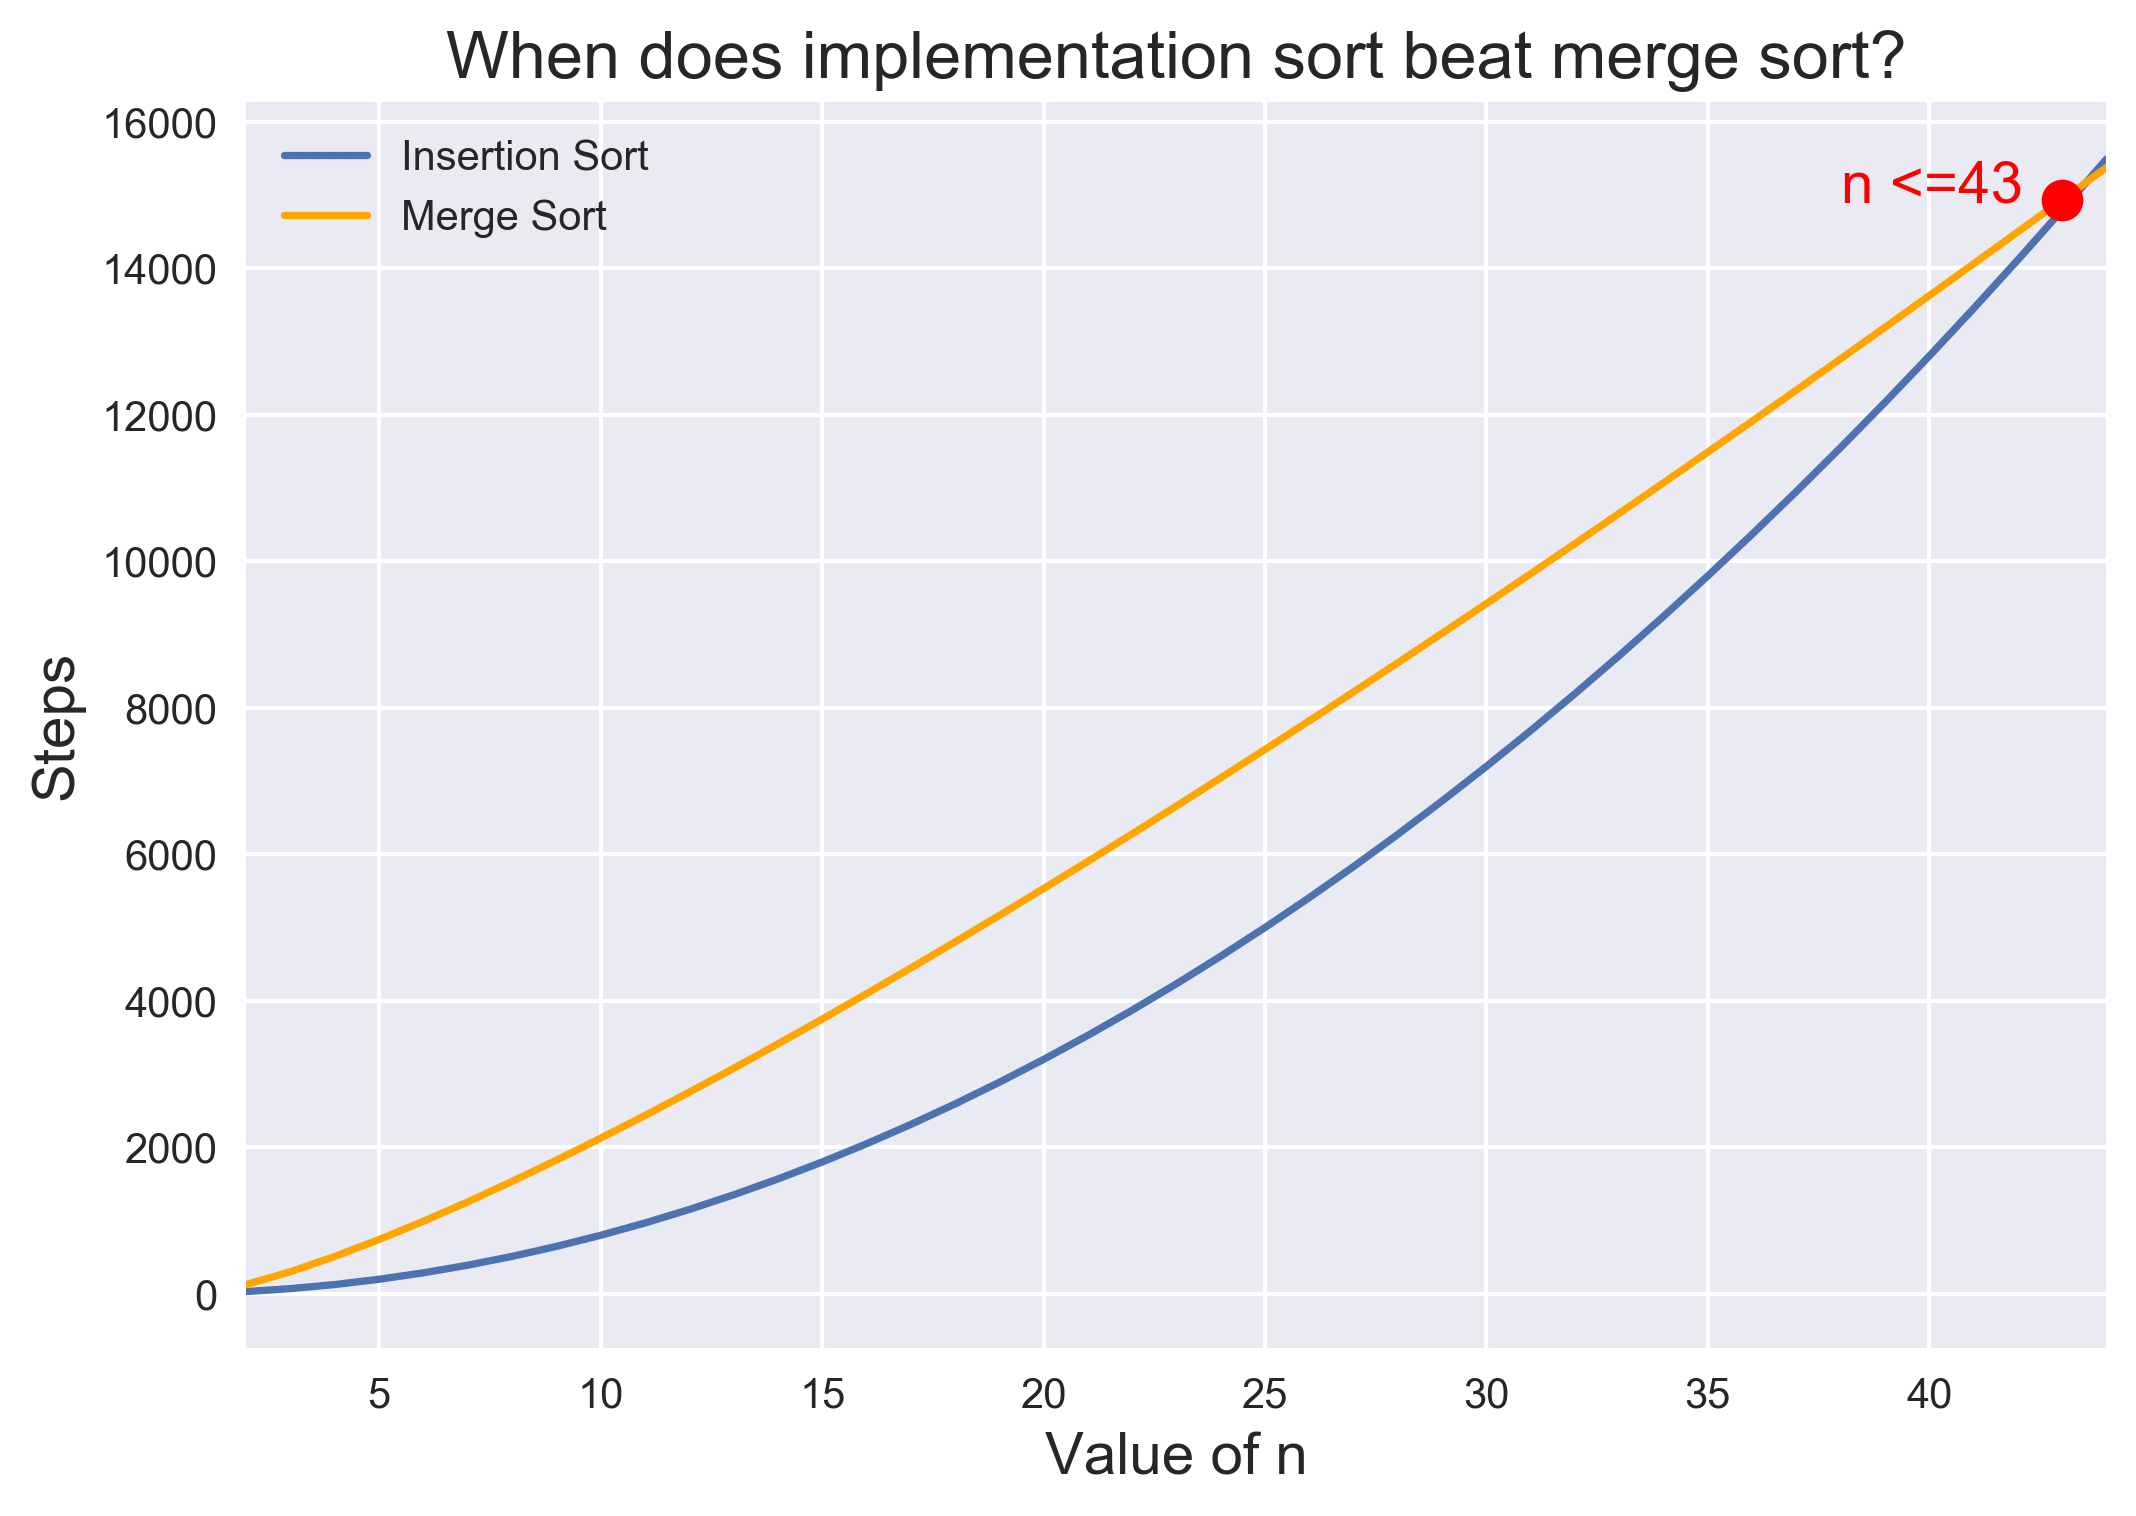
\includegraphics[scale=.65]{ques1.2-2.png}\\
\clearpage

\subsubsection*{Question 1.2-3}
What is the smallest value of $n$ such that an algorithm whose running time is 100$n^2$ runs faster than an algorithm whose running time is 2$^n$ on the same machine?\\

Equation: 100$n^2 \leq$ 2$^n$\\
\indent Solution: $n\geq15$ (see Python code)\\

\includegraphics[scale=.75]{sort_algo2.png}\\

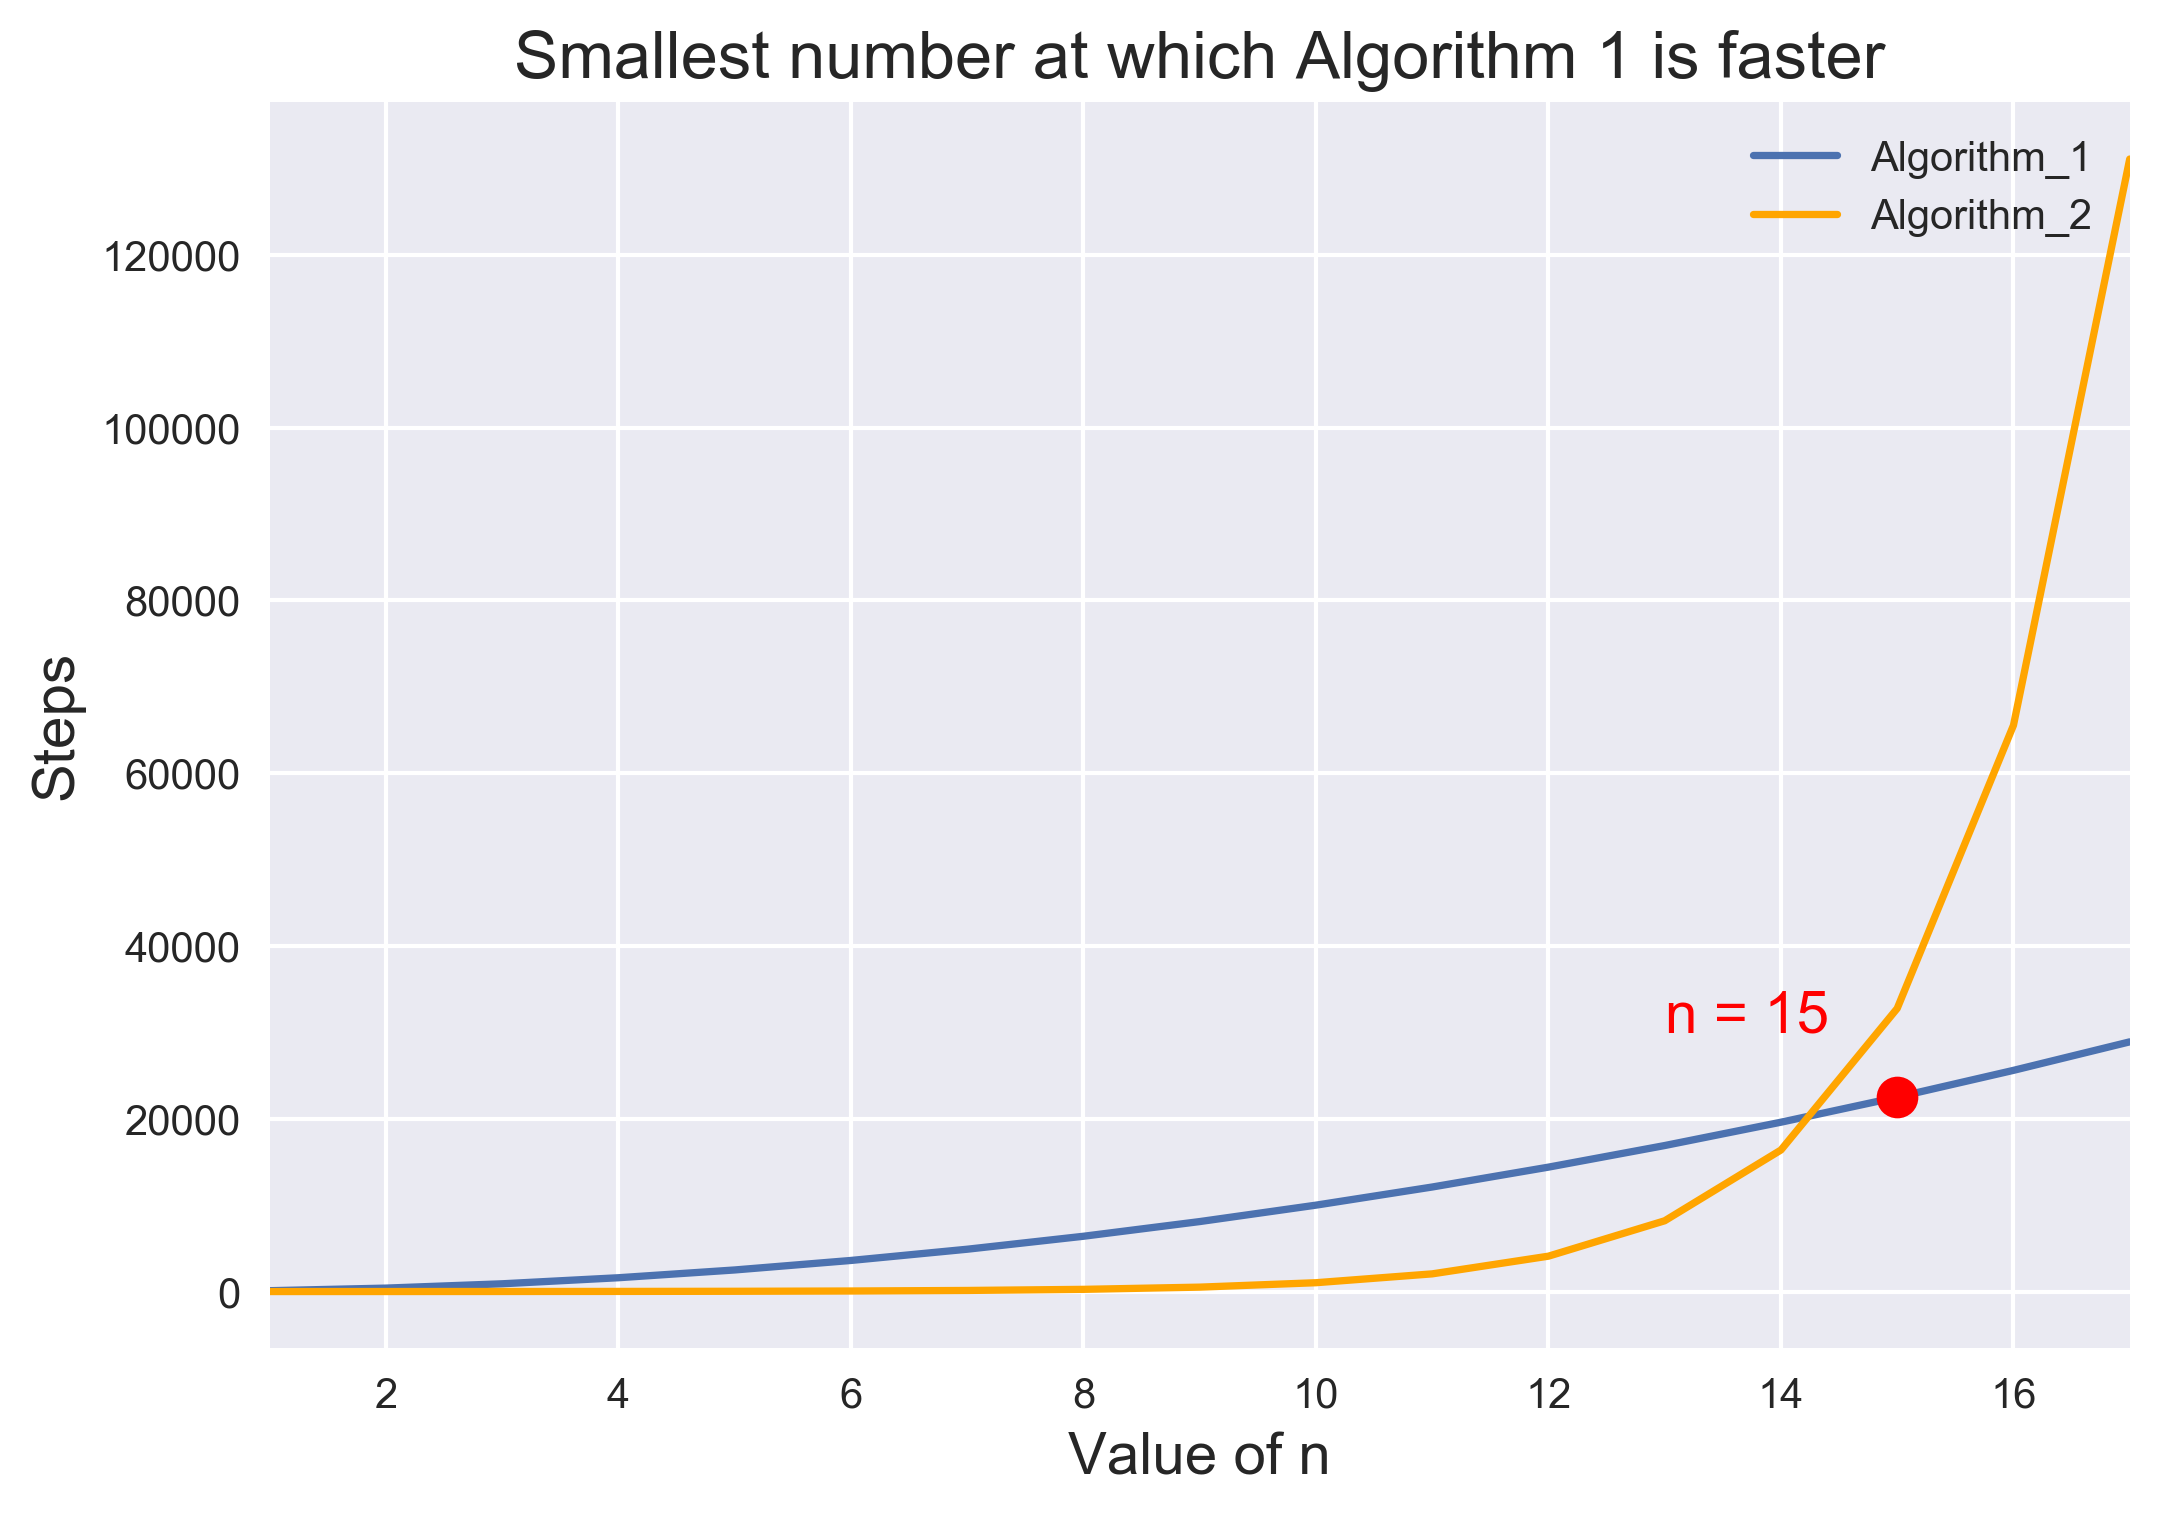
\includegraphics[scale=.65]{ques1.2-3.png}\\

\section*{Problems}\nointerlineskip
\noindent \rule{\linewidth}{0.01pt}
\subsubsection*{Problem 1-1}

For each function $f(n)$ and time $t$ in the following table, determine the largest size $n$ of a problem that can be solved in time $t$, assuming that the algorithm to solve the problem takes $f(n)$ microseconds.\\

(For solutions to $n$ log $n$ and $n$! refer to code in Python.)\\

 \noindent \begin{tabular}{|p{.8cm}|p{1.4cm}|p{1.6cm}|p{1.8cm}|p{1.8cm}|p{2cm}|p{1.8cm}|p{2.4cm}|}
\hline
 & 1 second & 1 minute & 1 hour & 1 day & 1 month &	1 year & 1 century \\
 \hline
 lg $n$ & $2^{10^6}$ & $2^{6\cdot10^7}$ & $2^{36\cdot10^8}$ & $2^{864\cdot10^{8}}$ & $2^{2592\cdot10^{9}}$ & $2^{31536\cdot10^{9}}$ & $2^{3.1536\cdot10^{15}}$ \\\hline
 $\sqrt{n}$ & $10^{12}$ & $36\cdot10^{14}$ & $1296\cdot10^{16}$ & $746496\cdot10^{16}$ & $6718464\cdot10^{18}$ & $994519296\cdot10^{18}$ & \small $9.9583\cdot10^{30}$\\\hline
$n$ & $10^6$ & $6\cdot10^7$& $36\cdot10^8$ & $864\cdot10^8$ & $2592\cdot10^9$ & $31536\cdot10^9 $& $3.1536\cdot10^{15}$ \\\hline
\small $n$ lg $n$ &  62746  &  2801417 &  \small 133378058 
& \small 2.7551 $\cdot 10^{9}$ 
& \small 7.1871 $\cdot 10^{10}$
& \small 7.9763 $\cdot 10^{11}$
& \small 6.8611 $\cdot 10^{13}$
\\\hline
$n^2$ & 1000 & 7745 & 60000 & 293938 & 1609968 &  5615692 &  56176151 \\\hline
$n^3$ & 100 & 391 & 1532 & 4420 & 13736 & 31593 & 146645 \\\hline
$2^n$ & 19 & 25 & 31 & 36 & 41 & 44 & 51 \\\hline
$n!$ & 9 & 11 & 12 & 13 & 15 & 16 & 17 \\\hline
\end{tabular}\\

\end{document}